%%%%%%%%%%%%%%%%%%%%%%%%%%%%%%%%%%%%%%%%%%%%%%%%%%%%%%%%
%%
\section{The cal\_DARK recipe}
\label{ch:the_recipes:cal_DARK_spirou}
%%
%%%%%%%%%%%%%%%%%%%%%%%%%%%%%%%%%%%%%%%%%%%%%%%%%%%%%%%%

Dark with short exposure time (~5min, to be defined during AT-4) to check if read-out noise, dark current and hot pixel mask are consistent with the ones obtained during technical night. Quality control is done automatically by the pipeline \\


% -------------------------------------------------------
\subsection{The inputs}
% -------------------------------------------------------
The input of \calDARK is as follows:
\begin{cmdbox}
cal_DARK_spirou.py  night_repository  filenames
\end{cmdbox}
\noindent for example:
\begin{cmdbox}[title={example}]
cal_DARK_spirou.py 20170710 dark_dark02d406.fits
\end{cmdbox}
\noindent or
\begin{pythonbox}
import cal_DARK_spirou
night_repository = '20170710'
filenames = ['dark_dark02d406.fits']
cal_DARK_spirou.main(night_repository, file=filenames)
\end{pythonbox}

\noindent where `night\_repository' defines \argnightname and `filenames' define the list of files in \argfilenames. All files in filenames must be valid python strings separated by a space (command line) or in a line (python). \\

\noindent Filename prefixes allowed are:
\begin{itemize}
	\item dark\_dark
\end{itemize}

% -------------------------------------------------------
\subsection{The outputs}
% -------------------------------------------------------
The outputs of \calDARK are as follows:

\begin{itemize}
\item \definevariable{text:darkfile}{darkfile} in form:
\begin{tcustomdir}
\{\reduceddir\}/\{date prefix\}\_\{file\}.fits
\end{tcustomdir}

\item \definevariable{text:darkbadpixfile}{darkbadpixfile} in form:
\begin{tcustomdir}
\{\reduceddir\}/\{date prefix\}\_\{file\}\_badpixel.fits
\end{tcustomdir}
\end{itemize}

\noindent where `date prefix' is constructed from \argnightname and the file name is the first file in \argfilenames. \\

\noindent For example for \reduceddir\lstinline[style=pythoninline]|='/drs/data/reduced/20170710'| and \argfilenames\lstinline[style=pythoninline]|=['dark_dark02d406.fits']| the output files would be:
\begin{tcustomdir}
\begin{itemize}
\item /drs/data/reduced/20170710/20170710\_dark\_dark02d406.fits
\item /drs/data/reduced/20170710/20170710\_dark\_dark02d406\_badpixel.fits
\end{itemize}
\end{tcustomdir}

% -------------------------------------------------------
\subsection{Summary of procedure}
% -------------------------------------------------------
\begin{enumerate}
\item adds defined `dark\_dark' files together
\item resizes the image
\item calculates the fraction of dead pixels [full, blue part, red part]
\item calculates median dark level [full, blue part, red part]
\item calculates threshold of dark level to retain
\item removes dead pixels by setting them to 0
\item does some quality control
\item updates calibDB with key "DARK"
\end{enumerate}


% -------------------------------------------------------
\subsection{Quality Control}
% -------------------------------------------------------


There are currently three quality control checks for cal\_DARK\_spirou
\begin{itemize}
\item Unexpected median dark level if: 
\begin{thighlight}
\begin{equation}
\text{Median Flux} > \text{\definevariable{text:qc_max_darklevel}{qc\_max\_darklevel}}
\end{equation}
\end{thighlight}

\item Unexpected fraction of dead pixels if: 
\begin{thighlight}
\begin{equation}
\text{Number of dead pixels} > \text{\definevariable{text:qc_max_dead}{qc\_max\_dead}}
\end{equation}
\end{thighlight}

\item Unexpected fraction of dark pixels if:
\begin{thighlight}
\begin{equation}
\text{Number of bad dark pixels} > \text{\definevariable{text:qc_max_dark}{qc\_max\_dark}}
\end{equation}
\end{thighlight}
\end{itemize}

\noindent If none of these quality control criteria are valid then the output file is passed into the \calibdb with key `DARK' for the `darkfile' and `BADPIX' for the `darkbadpixfile'. \\

\noindent For example the following lines are added to the \calibdb for 
\argnightname{\lstinline[style=pythoninline]| = "20170710" |} and \argfilenames{\lstinline[style=pythoninline]| = "dark_dark02d406.fits" |}. \\

\begin{textbox}[title={In calibration database file}]
DARK 20170710 20170710_dark_dark02d406.fits 2017-07-10-12:37:48.260000 1499690268.26
BADPIX 20170710 20170710_dark_dark02d406_badpixel.fits 2017-07-10-12:37:48.260000 1499690268.26
\end{textbox}

% -------------------------------------------------------
\newpage
\subsection{Example working run}
% -------------------------------------------------------

An example run where everything worked is below:
\begin{cmdbox}[title={example}]
cal_DARK_spirou.py 20170710 dark_dark02d406.fits
\end{cmdbox}
\begin{cmdboxprintspecial}[fontupper=\tiny]
@gHH:MM:SS.S -   || ***************************************** 
HH:MM:SS.S -   || * SPIROU \@(#) Geneva Observatory (VERSION) 
HH:MM:SS.S -   || ***************************************** 
HH:MM:SS.S -   ||(dir_data_raw)      DRS_DATA_RAW=/drs/data/raw 
HH:MM:SS.S -   ||(dir_data_reduc)    DRS_DATA_REDUC=/drs/data/reduced 
HH:MM:SS.S -   ||(dir_calib_db)      DRS_CALIB_DB=/drs/data/calibDB 
HH:MM:SS.S -   ||(dir_data_msg)      DRS_DATA_MSG=/drs/data/msg 
HH:MM:SS.S -   ||(print_level)       PRINT_LEVEL=all         %(error/warning/info/all) 
HH:MM:SS.S -   ||(log_level)         LOG_LEVEL=all         %(error/warning/info/all) 
HH:MM:SS.S -   ||(plot_graph)        DRS_PLOT=1            %(def/undef/trigger) 
HH:MM:SS.S -   ||(used_date)         DRS_USED_DATE=undefined
HH:MM:SS.S -   ||(working_dir)       DRS_DATA_WORKING=/drs/data/tmp/
HH:MM:SS.S -   ||                    DRS_INTERACTIVE is not set, running on-line mode
HH:MM:SS.S -   ||                    DRS_DEBUG is set, debug mode level:1
HH:MM:SS.S -   |ipython:2d406|Now running : ipython on file(s): dark_dark02d406.fits
HH:MM:SS.S -   |ipython:2d406|On directory /drs/data/raw/20170710
HH:MM:SS.S -   |ipython:2d406|ICDP_NAME loaded from: /drs/INTROOT/config/constants_SPIROU.py
HH:MM:SS.S - * |ipython:2d406|Correct type of image for dark (dark_dark)
HH:MM:SS.S - * |ipython:2d406|Now processing Image TYPE UNKNOWN with ipython recipe
HH:MM:SS.S -   |ipython:2d406|Reading Image /drs/data/raw/20170710/dark_dark02d406.fits
HH:MM:SS.S -   |ipython:2d406|Image 2048 x 2048 loaded
HH:MM:SS.S - * |ipython:2d406|Dark Time = 597.489 s
HH:MM:SS.S -   |ipython:2d406|Doing Dark measurement
HH:MM:SS.S - * |ipython:2d406|In Whole det: Frac dead pixels= 14.7 % - Median= 0.35 ADU/s - Percent[5:95]= 0.08-99.57 ADU/s
HH:MM:SS.S - * |ipython:2d406|In Blue part: Frac dead pixels= 1.0 % - Median= 0.15 ADU/s - Percent[5:95]= 0.09-0.53 ADU/s
HH:MM:SS.S - * |ipython:2d406|In Red part : Frac dead pixels= 20.5 % - Median= 2.11 ADU/s - Percent[5:95]= 0.18-232.09 ADU/s
HH:MM:SS.S - * |ipython:2d406|Frac pixels with DARK > 100.0 ADU/s = 4.3 %
@g@yHH:MM:SS.S - \@ |python warning|Line 138 warning reads: invalid value encountered in greater
@y@gHH:MM:SS.S - * |ipython:2d406|Total Frac dead pixels (N.A.N) + DARK > 100.0 ADU/s = 18.9 %
HH:MM:SS.S - * |ipython:2d406|QUALITY CONTROL SUCCESSFUL - Well Done -
HH:MM:SS.S -   |ipython:2d406|Saving Dark frame in 20170710_dark_dark02d406.fits
@g@yHH:MM:SS.S - \@ |python warning|Line 980 warning reads: Card is too long, comment will be truncated.
@y@gHH:MM:SS.S -   |ipython:2d406|Saving Bad Pixel Map in 20170710_dark_dark02d406_badpixel.fits
@g@yHH:MM:SS.S - \@ |python warning|Line 980 warning reads: Card is too long, comment will be truncated.
@y@gHH:MM:SS.S - * |ipython:2d406|Updating Calib Data Base with DARK
HH:MM:SS.S - * |ipython:2d406|Updating Calib Data Base with BADPIX
HH:MM:SS.S - * |ipython:2d406|Recipe ipython has been succesfully completed@g
\end{cmdboxprintspecial}


% -------------------------------------------------------
\newpage
\subsection{Interactive mode}
% -------------------------------------------------------


\noindent In interactive mode (\definevariable{text:drs_plot}{DRS\_PLOT} = 1) three figures will also appear (see Figure \ref{figure:cal_DARK_spirou}).


\begin{figure}

\begin{center}
\begin{minipage}{.495\textwidth}
\begin{center}
\includegraphics[width=\textwidth]{Figures/cal_DARK_spirou_1.pdf}
a
\end{center}
\end{minipage}%
\begin{minipage}{.495\textwidth}
\begin{center}
\includegraphics[width=\textwidth]{Figures/cal_DARK_spirou_2.pdf}
b
\end{center}
\end{minipage}%
\end{center}

\begin{center}
\begin{minipage}{.495\textwidth}
\begin{center}
\includegraphics[width=\textwidth]{Figures/cal_DARK_spirou_3.pdf}
c
\end{center}
\end{minipage}%
\end{center}

\caption{\textbf{(a)} The image with over-plot red and blue regions (red/blue rectangles). \textbf{(b)} The bad pixel mask, bad pixels have a value=1 (in black) and good pixels have a value=0 (in white). \textbf{(c)} Histograms of the image regions, the full image (in green), the blue section (in blue) and the red section (in red). \label{figure:cal_DARK_spirou}}
\end{figure}


